\chapter{Introduction}
This thesis aims to explore emotion recognition and its effectiveness in the Swedish language. With the rapid advancement of the technology industry and artificial intelligence, emotion recognition has started to play an increasingly important role in the enhancement of human-computer interactions. These areas hold potential to transform and develop several important fields, but there are still challenges in the field. Much of the research has been focused on specific languages, notably English. This research focuses on emotion recognition across two distinct modalities in Swedish, speech-based emotion recognition and text-based emotion recognition and aim to contribute to broadening the field of emotion recognition in a non-English language.

\section{Background}
According to Oatley et al. (2019), emotion recognition has attracted increasing attention with the rapid advancement of technology and artificial intelligence. Emotions are experienced by all humans but are difficult to define precisely. They are an internal experience that are foundational to our sense of identity, our relationships, and moral judgement. Scientists have faced challenges in the effort to characterize how emotions are communicated. Emotions are internal but also expressed externally through voice and movements of the body. They are not only communicated through the words we say, but also how we express them. Intonation is a source of varied emotional expressions where its states may alter patterns in vocalizations. It is considered that various emotion-related physiological changes influence acoustic features such as pitch, tempo, pitch variability, and loudness in the speech autocite{Oatley2019}. Beyond spoken signals, researchers have also developed a set of Natural Language Processing (NLP) techniques to interfer emotional states and opinions directly from text, based on methods at the intersection of artificial intelligence, computer science, and linguistics \autocite{Kansara2020}.
With the development of Artificial Intelligence several techniques have accelerated in the recent years, including for NLP, even if its origins back to the 1950s when questions about whether a machine could learn and think to interact with humans raised. \autocite{Alvarez2024}. NLP has remained as a significant contributor of AI. Some of the active research areas in the NLP domain is Machine Translation, Chatbots, recognizing speech, text summarization, and sentiment analysis \autocite{Kusal2023}. Figure \ref{fig:subdomains-AI} demonstrates the different subdomains of NLP. 
\begin{figure}[ht]
    \centering
    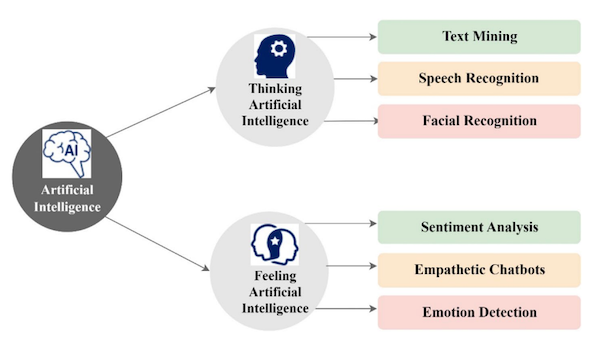
\includegraphics[height=7cm]{png/subdomains AI.png}
    \caption{\textit{Subdomains of NLP \autocite{Kusal2023}}.}
    \label{fig:subdomains-AI}
\end{figure}

Sentiment analysis is a computational branch in NLP that utilizes the detection and evaluation of people’s emotions, opinions, and moods based on text, speech, facial expression, etc., without analysis of these feelings \autocite{Ermakova2023}. The rise of sentiment analysis is associated with the growth of social media, which has generated vast amounts of digital option data recorded in digital forms. Since the early 2000’s, the field has become one of the most researched parts in NLP \autocite{Zhang2018}, expanding beyond computer science to fields like finance, marketing, political- and health science. Accordingly, sentiment analysis is valuable across different areas of society. Sentiment analysis is utilized in the popular index called the happy planet index \autocite{HappyPlanetIndex}, measuring sustainable well-being of different countries, even if it only can observe three feelings, positive, negative, or neutral. The happy planet index checks the happiness level calculated from a particular country, where emotion detection is used with sentiment analysis \autocite{Madhuri2021}.
With the evolution of deep learning networks, emotion detection has advanced \autocite{Safari2023}. Sentiment analysis identifying positive, negative, or neutral states have progressed into recognizing the six basic emotions; joy, sadness, anger, disgust, fear, and surprise in text. The emotions categorization fluctuate depending on the research. These basic six categories were determined by Paul Ekman \autocite{Oatley2019, Kusal2023} who determined that these six fundamental emotions is shared in people of different cultures, characterized by facial features. However, Ekman’s classification was made over 20 years ago when there was no agreement about which emotions should be considered as existed. Today, the agreement about evidence for universal emotional signals and evidence for five emotions is robust: anger, disgust, sadness, happiness, and fear \autocite{Ekman2016}.

Emotion recognition from textual data is important in various domains such as customer reviews, social media analysis, public monitoring, and conversational agents. A systematic review \autocite{Kusal2023} shows that Deep Learning models outperform traditional Machine Learning models due to their ability to capture contextual dependencies. The review further demonstrates the highest accuracy (76\%) is shown by transformer-based models such as bidirectional encoder representations from transformers (BERT), highlights challenges such as small or imbalanced datasets that can affect the model reliability, and notes that multimodal approaches with text, speech, and images improve emotion recognition \autocite{Madhuri2021}. However, text-based emotion detection (TBED) has challenges with identifying hidden emotions, and adapting to diverse languages. Datasets based on different languages than English, as Arabic and Hindi, are tested in a study \autocite{Maruf2024} that identifies challenges as limited resources for non-English languages. The authors underscore the potential of TBED but notes limitations as it is no universal solution for challenges like sarcasm, dynamic emotions, and cultural variances.

Emotion detection research progressed with Speech Emotion Recognition (SER) \autocite{Kusal2023}. It has shown that hearers can evaluate five emotions in speech-prosody, anger, happiness, sadness, fear, and tenderness, with 70 percent accuracy \autocite{Oatley2019}. Speech emotion recognition focuses on how something is said rather than the words themselves. Acoustic features like amplitude, formants, and pitch help classify emotions. Those features offer invaluable insights into the subtle emotional expressions conveyed through speech, assisting the complicated process of emotion recognition \autocite{Lian2023}.

Several studies distinguish different emotions through vocal features. Already in 2005, automatic recognition of positive and negative emotions in spoken dialogs was investigated \autocite{ChulMinLee2005}. In that study, acoustic, lexical, and discourse information were combined to enhance emotion detection and move beyond traditional acoustic-only ways. The authors analysed acoustic features, lexical features, and discourse features. Linear Discriminant Classifiers were used and resulted in good performance for acoustic and lexical information. A study by Bänziger et al. (2014) demonstrated that human listeners could reliably rate emotional expressions in acted voices. These human judgements had higher accuracy for detection of certain emotions, such as happiness, compared to technical analyses of acoustic measurements. 

According go \textcite{Khalil2019}, acoustic features enable emotion recognition through speech using deep learning, which offers many advantages over traditional sentiment-analysis methods. Deep learning models has the capability to automatically detect complex patterns and varying features without requiring manual feature extraction. The goal of speech emotion recognition (SER) is identification of emotions in speech, unrelated to the semantic content \autocite{Kusal2024}. Figure \ref{fig:blockdiagram-SER} represents a SER system.

\begin{figure}[ht]
    \centering
    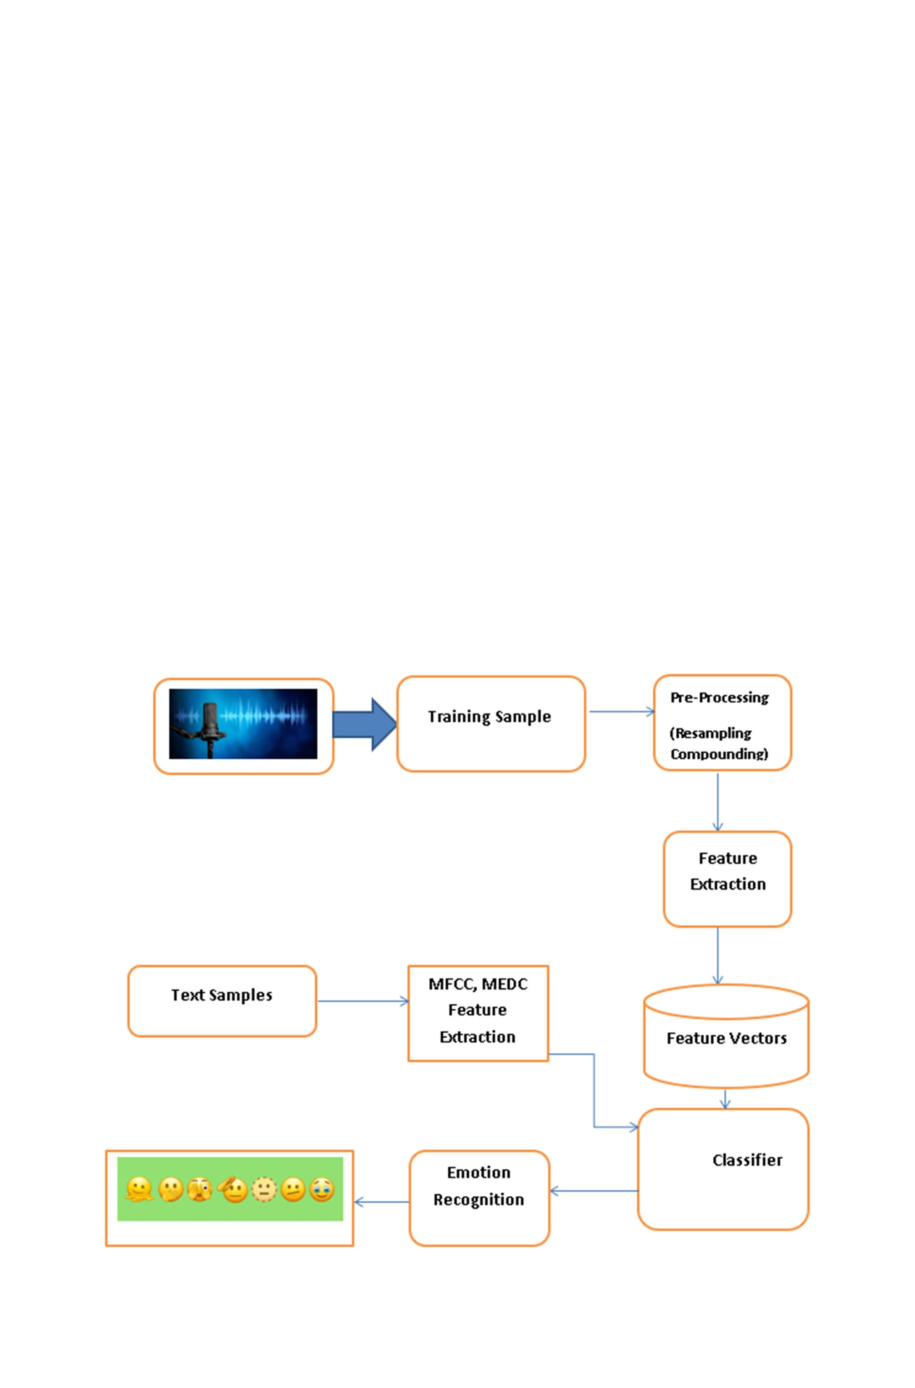
\includegraphics[height=7cm]{png/background/block-diagram.pdf}
    \caption{\textit{Block diagram of SER \autocite{Tyagi2024}.}}
    \label{fig:blockdiagram-SER}
\end{figure}

In recent years, speech emotion recognition has emerged as a research area driven by its applications in human-computer interaction \autocite{Zhang2021}. The advancements has led to the development of intelligent affective services in fields such as call centres, healthcare, surveillance, and affective computing. The accuracy of models tested in recent years have improved significantly \autocite{Adebiyi2024, Praseetha2022, Rahman2024}.  Several studies conducted in the last year’s show emotion detection accuracy results over 90\%. 

\textcite{Juslin2018} concluded a study in 2018 analysing 1,877 voice clips from 23 datasets to compare spontaneous and posed emotions. Their findings highlighted key differences: 
\begin{itemize}
    \item Spontaneous expressions were rated as more genuine than posed ones, even when intensity was controlled. 
    \item Posed expressions were more intense, but intensity alone did not fully explain perceived authenticity. 
    \item Acoustic differences were small but present, mainly in pitch range, speech rate, and voice intensity. 
    \item Highly intense spontaneous emotions conveyed emotions as clearly as posed ones, suggesting that emotion intensity plays a role in perception. 
\end{itemize}
These findings underscore that posed and spontaneous emotions are not interchangeable and that SER datasets must distinguish between these sample types to build models that can generalize to real-world emotional speech accurately.  

One recent review of SER corpora and features \autocite{Rathi2024} shows that most studies still target only six emotions—happiness, anger, sadness, surprise, fear, and neutrality—even though narrower sets (e.g.\ anger, fear, happiness, sadness) dominate earlier work \autocite{Scherer2018}. In contrast, GoEmotions is a large, detailed text database for 27 distinct emotions, a study by \textcite{Demszky2020} obtained an average F₁ of 0.46 (0.86 for gratitude, 0.00 for grief) and 0.64 when reduced to six labels. While this GoEmotions-study is included in the research behind the commercial system Hume.ai, and highlights the value of fine-grained emotion categories \autocite{HumeAI-AboutHume}, which is important to acknowledge since because of potential biases.  

Datasets drive both speech- and text-based emotion models.  Speech emotion recognition datasets are gathered in three ways, acted by performers, induced in controlled settings, or from natural conversations, affecting how expressive and realistic the recordings are. \textcite{Rathi2024} analysed 93 research papers where IEMOCAP and RAVDESS are among the most widely used datasets, chosen by 35.83\% and 21.50\% of researchers, respectively. They further state that dataset choice, recording conditions, and selected features (e.g. MFCCs, pitch, intensity, prosody) impact SER accuracy significantly, and that natural speech is more difficult to classify due to its high variability and background noise.

The number of natural datasets is relatively limited \autocite{Cai2023}, and many research papers test on acted datasets. For example, the empirical analysis \textcite{Ahammed2024} demonstrates a high-accuracy SER system (100\% accuracy, precision, and F1-score) on a combined RAVDESS, TESS, and SAVEE dataset. Each dataset includes posed or elicited emotions in English speech. Similarly, different models for SER achived over 94\% accuracy for these same acted datasets \autocite{Alroobaea2024}. However, spontaneos speech is not validated in these studies and depends on acted data. 

In contrast, Text-Based Emotion Detection (TBED) are driven by diverse text datasets, from six emotions to GoEmotions set with 27 emotions \autocite{Kusal2023}. Researchers in TBED can use publicly available datasets with reliable annonating, for instanse derieved from stories, publications, news, social media texts, or reviews on movies. According to \textcite{Kusal2023}, many datasets are based on social media, including casual writing style which is a big challenge. The use of short messages and informal language has limited research. Human emotion expressions and the texts conveying them are ambiguous and subjective, additionally, emotions are multifaceted with varying expressions. Therefore, the authors claim that human mapping is important. Over 3.5 milliom self-labeled posts on Twitter was used to train a model in \textcite{Lee2023} , achieving up to 0.87 F1 on human-annonated sets and 0.79 F1 on self-reported hashtags. However, like SER, TBED is dominated by English and lacks large, natrualistic datasets in other languages. 

The promising development of emotion recognition has been adapted in research for other areas than computer and machine learning science. SER is beneficial in translating languages, interactive courses and tutorials held online where the student’s emotional state can be understood to help the machine make decisions on how to present the course \autocite{Abbaschian2021}. It can be implemented in vehicles’ safety structures to recognize the driver’s emotional state and therefore prevent accidents. 

Several studies \autocite{DeSouza2021, Drougkas2024, Simcock2020,Singh2023} demonstrate the potential benefit of AI-based emotion recognition in mental health, investigating it can assist psychiatrics diagnosing and identifying potential mental illnesses. \textcite{DeSouza2021} showed how leveraging speech and text analysis with NLP can help detect late-life depression and predict its severity with 86-92\% accuracy.
\textcite{Drougkas2024} compared unimodal approaches, either text- or audio-based and combined audio-text models, resulting in text unimodal accuracy between 78\% and 87\% with F1 scores from 0.60 to 0.79, audio unimodal accuracy of 64\%-72\% with F1 values as low as 0.0 up to 0.46. Multimodal approaches, combining text and audio, showed similar accuracy (80\% - 87\%) and F1 scores (0.60-0.80) as text-unimodal approaches. The authors conclude that text model outperform the acoustic model in recognising mental health indicators, but that multimodal models can outperform unimodal techniques since positive F1 scores increase combining the models. 

In summery, speech emotion recognition is proficient in capturing vocal cues, especially on acted datasets, while text-based emotion detection relies on transformer models trained on large text collections. However, most research is based on English and uses acted or social-media data, with few studies exploring natural, spontaneous speech or on other languages.  


\section{Problem Description}
Despite significant progress in speech emotion recognition, there are limitations in current research. For instance, emotional voice samples are usually obtained from actors portraying emotions using scripted speech. These acted expressions tend to be more intense and exaggerated than naturally occurring emotions. However, this method risks overemphasizing obvious emotional cues while missing subtle ones. It is argued that such portrayals reflect social norms more than genuine physiological responses, although all public expressions may involve some degree of performance \autocite{Scherer2018}.

The way emotional speech data is collected depends on the design and purpose of the SER system. As datasets shift from acted emotions to more spontaneous or real-life emotions, emotion recognition becomes more challenging. Many researchers prefer acted emotion datasets because they offer a wide range of emotions and large amounts of data \autocite{Rathi2024}. Induced datasets are collected by constructing an artificial emotional situation, without the knowledge of the performer or speaker. This results in a more naturalistic database, but issues regarding ethics may apply, since the speaker should know they have been recorded for research \autocite{Khalil2019}. 

Estimation of emotions from spontaneous speech is a challenging task. Most studies test models on acted datasets \autocite{Khalil2019, Ahammed2024, Praseetha2022, Alroobaea2024}. The primary reason for the concentration on acted SER tasks is that acted emotions can be easily performed in a controlled laboratory setting, often resulting in high SER accuracy. However, these emotions tend to be exaggerated and may not accurately reflect how emotions are expressed in real-world situations. Consequently, detecting spontaneous emotions in natural environments is significantly more complex and challenging compared to recognizing acted emotions \autocite{Zhang2021}. Figure \ref{fig:databases-diff} demonstrates the difficulty level for varying settings.

\begin{figure}[ht]
    \centering
    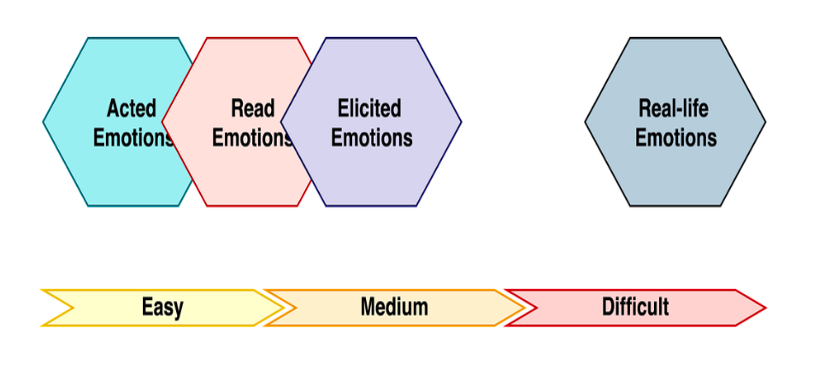
\includegraphics[height=6cm]{png/databases difficulty.png}
    \caption{\textit{Emotion recognition databases and their difficulty level \autocite{Khalil2019}.}}
    \label{fig:databases-diff}
\end{figure}

Text-Based Emotion Detection (TBED) shows similar gaps regarding the data the majority of the researched models are trained and evaluated on. Although transformer models reach up to 76 \% accuracy on
English datasets \autocite{Kusal2023}, they are heavily dependent 
on informal social-media or review texts. Moreover, TBED resources for other languages is limited,  
and challenges like sarcasm and cultural nuance affects the reliability of the models \autocite{Maruf2024,Lee2023}.

The Swedish language is not widely spoken and therefore very limited research has been concluded on the Swedish speech. One study \autocite{Ekberg2023} investigated Swedish emotion recognition through feature extraction and concluded that emotions in Swedish speech have unique sound patterns. The emotion results showed that surprise is a very distinct emotion, but happiness and anger sound alike, which could confuse listeners. 

Limitations as overreliance on acted English data, lack of natrual and non-English datasets, and modality-specific biases, are motivations for this thesis. We will compare SER and TBED in Swedish, using both speech and text from the same speakers and explore the alignment against their self-reported emotions to test real-world performance. 

\newpage
\section{Purpose and Research Questions}

The advancement of artificial intelligence (AI) has significantly improved the ability to recognize human emotions, both through speech and text. This offers transformative potential across domains such as mental health, education, and human-computer interaction. Speech Emotion Recognition (SER) and Text-based emotion detection (TBED) have become key areas within the field of Natural Language processing (NLP), leveraging deep learning to interpret different emotional cues with increasing accuracy. However, despite these advancements, significant challenges remain in ensuring that emotion recognition systems are robust, culturally inclusive, and reflective of real-world emotional expressions. Much of the existing research relies on acted datasets, which may underperform when it comes to subtle, spontaneous emotions in everyday contexts, and there is a notable gap in understanding how these models perform across diverse linguistic and cultural situations, such as the Swedish language. The number of studied languages is not that broad, and the studies on accuracy for a new language implies that more research on the generalizability to other languages is essential. Furthermore, while speech and text offer complementary perspectives on emotions, their alignment with individuals own perceptions of their emotions remains unexplored. 

This study aims to address the dataset gap by investigating the performance of AI-driven emotion recognition systems in a specific context: Swedish speech and its transcribed textual content. By focusing on Swedish – a language with limited prior research in SER – this thesis seeks to contribute to a broader understanding of how linguistic and cultural factors can influence emotion recognition, which is applicable to multilingual understanding for emotion recognition for different languages. Additionally, the integration of speech and text analysis gives an opportunity to explore multimodal approaches. The alignment between AI-generated emotion labels and self-reported emotions is an overlooked area. 
Although emotions are inherently difficult to define and can be challenging for individuals to self-assess, it is valuable to examine the alignment between model outputs and people’s own perceieved emotions. Publicly available AI models and APIs, despite their use in real-world applications, are rarely compared agaisnt such subjective human data, making this comparative evaluation both novel and scientifically signficiant. 

The purpose of this thesis is therefore to evaluate how the Llama-3 model from NLP Cloud and Hume AI recognizes emotions from Swedish speech, to assess whether its transcribed textual content can convey emotional states independently and compare these AI-generated labels with self-reported emotions from Swedish speakers. By addressing the specific challenge of emotion recognition in a less-studied language, the study contributes to the broader scientific discussion on emotion-recognitions generalizability. The study will provide insights into alignment between speech and text modalities, cultural emotional expression, and the alignment between AI outputs and human experience.  

To explore speech emotion recognition for Swedish speech, vocal markers from Swedish speech recordings will be extracted and compared to a prior study \autocite{Ekberg2023}. With the usage of this research, the performance of an AI model for Swedish can be compared, and therefore the first research question of this study is: 

\begin{quote}
\textit{[1] How does an AI model for speech recognition compare to research on vocal markers for emotions in Swedish speech?} 
\end{quote}
Text-based emotion recognition is a commonly used research field, but mostly for English text. To address this, it is interesting to assess whether transcribed Swedish speech can reveal emotions independently, which leads to the second research question: 
\begin{quote}
    \textit{[2] What similarities and differences emerge between emotions detected from audio features and from the textual transcripts of the same speech data? }
\end{quote}
The perception of emotions is a complex field, with few studies made on the alignment between machine-labeled emotions and human-perceived emotions. To undertake this, its comparison will be explored in the third research question:  
\begin{quote}
    \textit{[3] How do AI-generated emotion labels (speech \& text-based) compare to self-reported emotions?}
\end{quote}

\section{Scope and Limitations}
The scope focuses on AI-based emotion recognition in Swedish speech and text, considering its constraints in design and resources. The study explores challenges like reliance on acted datasets, language differences, and the alignment between AI predictions compared to self-reported emotions. Since this is an exploratory thesis, some limitations are recognized but accepted for feasibility. 
\subsection{Scope}
The study evaluates AI-driven emotion recognition in Swedish, a language with little prior research in this area. It analyses emotions from about 15 Swedish-speaking participants through short interviews designed to evoke natural emotions. 
Particpants, both male and female, have varying age from 20-78 years. 
The study includes: 
\begin{itemize}
    \item \textbf{Vocal Extraction: } With Praat Parselmouth, a Python library for Praat software used for feature extraction from audio recordings. 
    \item \textbf{Speech-based analysis:} Using Hume.ai \autocite{HumeAI-AboutHume}, an API with AI-based emotion recognition in speech for AI-based speech emotion recognition. 
    \item \textbf{Text-based analysis:} Using NLP Cloud \autocite{NLPCloud}, an API utilizing AI to transcribe speech and detect emotions from text.
    \item \textbf{Comparison with self-reports:} Participants rate their emotions on a scale of 1-6 (1 = very weak, 6 = very strong), compared to AI-generated labels. 
\end{itemize}
To keep this study manageable, it focuses on two semantic orientations, one positive and one negative designed interview for each participant. Five emotions are derieved from the audio and are reported by the participants.

The analysis relies on existing AI tools and API’s \autocite{HumeAI-AboutHume, NLPCloud} and Praat software for voice feature extraction, without developing new models. A mixed method is used, combining AI outputs with qualitative insights.

\subsection{Limitations}
Several factors limit the study’s depth and generalizability. With only 16 participants, the dataset is limited, and the results may not apply to all Swedish speakers as well as the findings may not apply beyond Swedish. The interviews are designed to elicit emotions and may not fully capture natural emotional responses, since they are partially induced, and the very nature of the interview setting cannot be directly applicable to real-world environments. The design of the emotion-eliciting scenarios may not be optimal because of deficient psychological expertise, even if the scenarios are based on prior research. By the same reason, the composition by the self-reports could be a limitation in combination with the subjectivity of participants’ emotion reports, that may be influenced by personal biases or recall inaccuracies. The selected emotion categories, commonly used in prior research, include more negative (anger, fear, sadness) than positive (joy) oriented emotions, leading to potential limitations on self-reports. Focusing on these emotions may exclude other relevant emotional states, as Hume AI’s output in fact cover several more emotion labels. Pre-trained AI models are utilized without modifying their algorithms, which may introduce biases. The study does not include biometric data, which could provide additional insights. For vocal extraction, Praat Parselmouth is applied, which in our implementation, does not cover the full set of vocal features included in the Swedish research \autocite{Ekberg2023} used for comparison in RQ1. 

These limitations are necessary compromises for feasibility within the study’s timeframe and resource constraints. The study does not aim to develop new AI models or solve all SER challenges. Instead, it provides initial insights into Swedish emotion recognition, tests existing AI tools, and identifies areas for future research. 

\section{Disposition}
From here, the report is structured as follows: 

\textbf{Theoretical Framework:} This chapter explores the underlying theories relevant to this study. It provides an overview of Natural Language Processing (NLP), Speech Based Emotion Recognition (SER), Hume.ai, Praat Parselmouth, Text-Based Emotion Recognition (TBED), NLP Cloud, and theories behind vocal markers in speech. The experiment is explained with relevant research for the interviews used for this study. 

\textbf{Method and Implementation:} This section introduces explanatory mixed method, experimental approach used to answer the research question. It describes the experimental setup, data collection process, methods of analysis, and considerations regarding validity and reliability.   

\textbf{Results:} Presents the collected data and analyses of the research questions. 

\textbf{Discussion:} Discussion for each research question and the methodology. 

\textbf{Conclusion:} Overall conclusion of the study, with key findings, implications and future research recommendations.  




